\documentclass[onecolumn, draftclsnofoot,10pt, compsoc]{IEEEtran}
\usepackage{url}
\usepackage{tabu}
\usepackage{color}    % colors for code listings
\usepackage{float}
\usepackage{caption}
\usepackage{geometry}
\usepackage{graphicx}
\usepackage{listings} % code listings
\usepackage{pdfpages} % for inserting pdfs into LateX
\usepackage{pgfgantt}
\usepackage{setspace}

\graphicspath{{images/}}
\geometry{textheight=9.5in, textwidth=7in, margin=0.75in}

%%%%%%%%%%%%%%%%%%%%%%%%%%%%%%%%%%%%%%%%%%%%%%%%%%%%%%%%%%%%%%%%%%%%%%%%%%%%%%%%%%%%%%%%%%%%%%%%%%%
% Code listing options %
\definecolor{mygreen}{rgb}{0,0.6,0}
\definecolor{mygray}{rgb}{0.5,0.5,0.5}
\definecolor{mymauve}{rgb}{0.58,0,0.82}

\lstset{ 
  backgroundcolor=\color{white},   % choose the background color
  basicstyle=\footnotesize,        % size of fonts used for the code
  breaklines=true,                 % automatic line breaking only at whitespace
  captionpos=b,                    % sets the caption-position to bottom
  commentstyle=\color{mygreen},    % comment style
  escapeinside={\%*}{*)},          % if you want to add LaTeX within your code
  keywordstyle=\color{blue},       % keyword style
  stringstyle=\color{mymauve},     % string literal style
}
\lstdefinestyle{customc}{
  belowcaptionskip=1\baselineskip,
  breaklines=true,
  frame=L,
  xleftmargin=\parindent,
  language=C,
  showstringspaces=false,
  basicstyle=\footnotesize\ttfamily,
  keywordstyle=\bfseries\color{mygreen},
  commentstyle=\itshape\color{mygreen},
  identifierstyle=\color{blue},
  stringstyle=\color{orange},
}
%%%%%%%%%%%%%%%%%%%%%%%%%%%%%%%%%%%%%%%%%%%%%%%%%%%%%%%%%%%%%%%%%%%%%%%%%%%%%%%%%%%%%%%%%%%%%%%%%%%
% 1. Fill in these details
\def \CapstoneTeamName{     TeamName}
\def \CapstoneTeamNumber{       24}
\def \GroupMemberOne{            Ciin S. Dim}
\def \GroupMemberTwo{           Louis Leon}
\def \CapstoneProjectName{      Kinect Based Virtual Therapy Solution}
\def \CapstoneSponsorCompany{   OSU Healthcare Systems Engineering Lab}
\def \CapstoneSponsorPerson{        Mehmet Serdar Kilinc}

% 2. Uncomment the appropriate line below so that the document type works
\def \DocType{      %Problem Statement
                %Requirements Document
                %Technology Review
                %Design Document
                Final Report
                }
            
\newcommand{\NameSigPair}[1]{\par
\makebox[2.75in][r]{#1} \hfil   \makebox[3.25in]{\makebox[2.25in]{\hrulefill} \hfill        \makebox[.75in]{\hrulefill}}
\par\vspace{-12pt} \textit{\tiny\noindent
\makebox[2.75in]{} \hfil        \makebox[3.25in]{\makebox[2.25in][r]{Signature} \hfill  \makebox[.75in][r]{Date}}}}
% 3. If the document is not to be signed, uncomment the RENEWcommand below
\renewcommand{\NameSigPair}[1]{#1}

%%%%%%%%%%%%%%%%%%%%%%%%%%%%%%%%%%%%%%%%%%%%%%%%%%%%%%%%%%%%%%%%%%%%%%%%%%%%%%%%%%%%%%%%%%%%%%%%%%%
\begin{document}
\begin{titlepage}
    \pagenumbering{gobble}
    \begin{singlespace}
        %\includegraphics[height=4cm]{coe_v_spot1}
        \hfill 
        % 4. If you have a logo, use this includegraphics command to put it on the coversheet.
        %\includegraphics[height=4cm]{CompanyLogo}   
        \par\vspace{.2in}
        \centering
        \scshape{
            \huge CS Capstone\DocType \par
            {\large Spring Term}\par
            {\large\today}\par
            \vspace{.5in}
            \textbf{\Huge\CapstoneProjectName}\par
            \vfill
            {\large Prepared for}\par
            \Huge \CapstoneSponsorCompany\par
            \vspace{5pt}
            {\Large\NameSigPair{\CapstoneSponsorPerson}\par}
            {\large Prepared by }\par
            Group\CapstoneTeamNumber\par
            % 5. comment out the line below this one if you do not wish to name your team
            %\CapstoneTeamName\par 
            \vspace{5pt}
            {\Large
                \NameSigPair{\GroupMemberOne}\par
                \NameSigPair{\GroupMemberTwo}\par
            }
            \vspace{20pt}
        }
        \begin{abstract}
        % 6. Fill in your abstract    
        The purpose of this document is to compile all of the documentation written for this project since Fall term. This includes an introduction to the project, requirements document, design document, technology review, weekly blog posts, expo poster, project documentation, recommended technical Resources for learning more, and conclusions and reflections.
    \end{abstract}     
    \end{singlespace}
\end{titlepage}
\newpage
\pagenumbering{arabic}
\tableofcontents
% 7. uncomment this (if applicable). Consider adding a page break.
\listoffigures
%\listoftables
\clearpage

% 8. now you write!
\section{Purpose}
The purpose of the Kinect Based Physical Therapy Solution project is to provide a solution for physical therapy patients diagnosed with Parkinson's disease to perform in-home therapy exercises. This solution will not only allow for an interactive way of completing a patient's required home therapy but will provide a way for their physical therapist to track their progress and monitor their exercises.

\section{Goals}
Our project will have a simple UI that can be easily navigated by a user with Parkinson's Disease. From the UI, the user will be able to select the option that allows them to select and do the available exercises. Our goal is to have two different exercises available to the user to choose from. One of our stretch goals is to be able to have a physical therapist prescribe exercises and specify frequency. The program will guide the user through these exercises using text and verbal instructions. One of our stretch goals is to implement visual (graphical) cues (over-laying their body on the camera feed) to the user to guide them through exercises. As the user performs exercises, their node data will be collected to be sent to their physical therapist as a .csv file, and it will be used for report generation. We will define the exercise's correct movements and compare them to the user's node data. This is how we will analyze the data to determine user accuracy for report generation. Another option the user will be able to select is report generation. This will display the user's performance data in graphs and charts, showing their progress with the exercises over time \cite{csvFile, Gestures}. 

\section{Project Introduction}
\subsection{Project Information}
The Kinect Based Physical Therapy project was requested by the OSU Healthcare Systems Engineering Lab, specifically by our client Dr. Mehmet Serdar Kilinc. The Healthcare System Engineering Lab in OSU is a research center which focuses on innovative non-traditional healthcare models, information technology healthcare interventions, and translational research. The lab is currently focusing on research projects that require sensor-based healthcare solutions. This project was specifically focused on using a Microsoft Kinect Sensor with the assumption being it could be useful for in-home health monitoring applications.

The importance of this project was to demonstrate a proof of concept that helps people with neurodegenerative conditions such as Parkinson's Disease get access to physical therapy remotely without the need for in-person therapy sessions. Access to physical therapy clinics is problematic due to physical disability that inhibits traveling and can be costly for patients. Non-wearable sensor-based solutions have the potential to reduce the number of in-person visits and the long-distance traveling that is required. 

\subsection{Team Members}
The two members of the development team for this project were Louis Leon and San Dim Ciin, two senior Computer Science students at Oregon State University. They both held the role as lead developers for this project. Each team member had large tasks in all the components of the project which ranged from building the user interface to automating the report generation process. The project's client, Dr. Kilinc supervised the project's direction and progress. He provided feedback at various stages of the development process and requested features that could serve as additions to the project overall. 
%%%%%%%%%%%%%%%%%%%%%%%%%  REQUIREMENTS DOCUMENT  %%%%%%%%%%%%%%%%%%%%%
\section{Requirements}

\includepdf[pages=-, pagecommand={}]{requiredDocuments/Requirements}  

\subsection{Requirement Changes}
*Add (your client should have okay'd): What new requirements were added? What existing requirements were changed? What existing requirements were deleted? Why?* 
\subsection{Final Project Timeline}
*Add: Final Gantt Chart as a record of what happened when.* 

%%%%%%%%%%%%%%%%%%%%%%%%%%  DESIGN DOCUMENT  %%%%%%%%%%%%%%%%%%%%%%%%%%
\section{Design}

\includepdf[pages=-, pagecommand={}]{requiredDocuments/DesignDocument}  

\subsection{Design Changes}
*Add (your client should have okay'd): What design aspects were changed, deleted or added? Why?*

%%%%%%%%%%%%%%%%%%%%%%  TECHNOLOGY REVIEW DOCUMENTS  %%%%%%%%%%%%%%%%%%
\section{Technology Review}

\includepdf[pages=-, pagecommand={}]{requiredDocuments/leonl_techReview}

\includepdf[pages=-, pagecommand={}]{requiredDocuments/dimc_techReview}
%%%%%%%%%%%%%%%%%%%%%%%%%%  TEAM WEEKLY BLOGS  %%%%%%%%%%%%%%%%%%%%%%%%
\section{Team Blog}
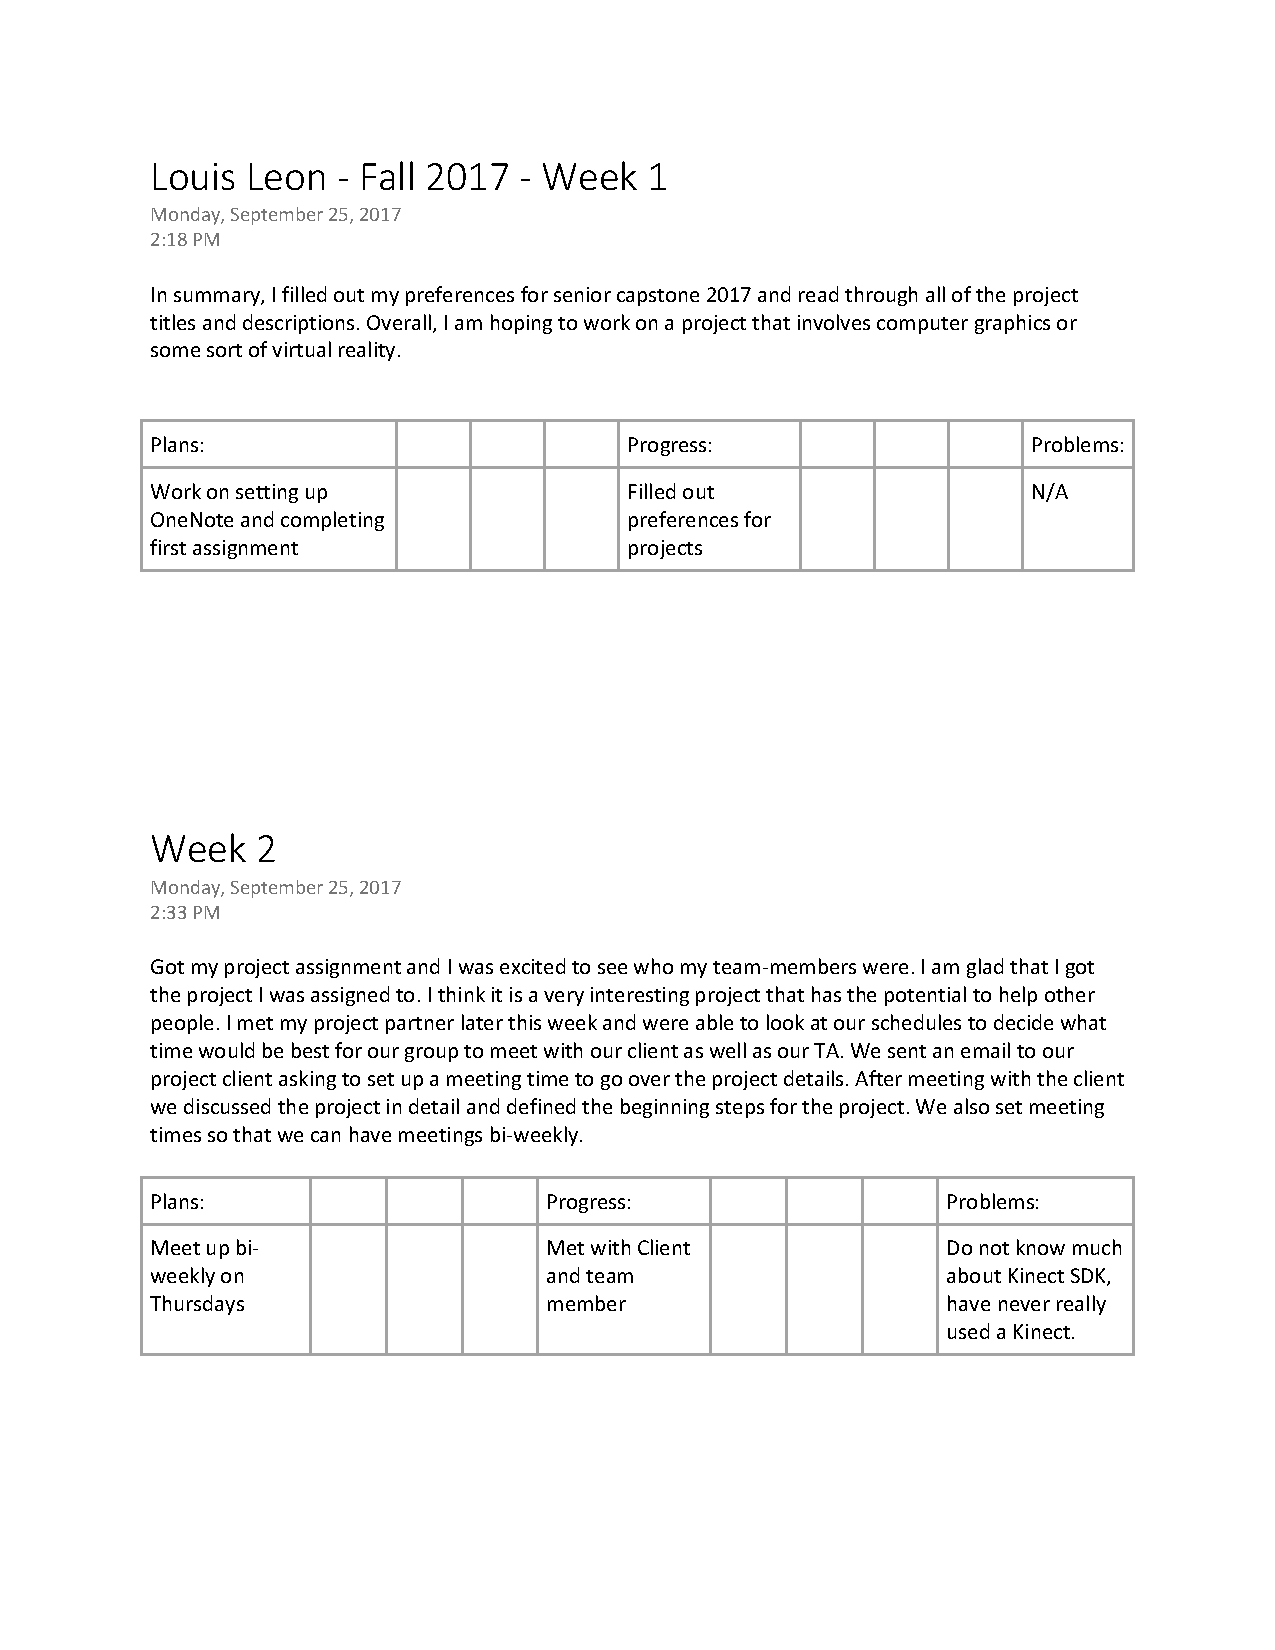
\includepdf[pages=-, pagecommand={}]{requiredDocuments/leonl_blog}
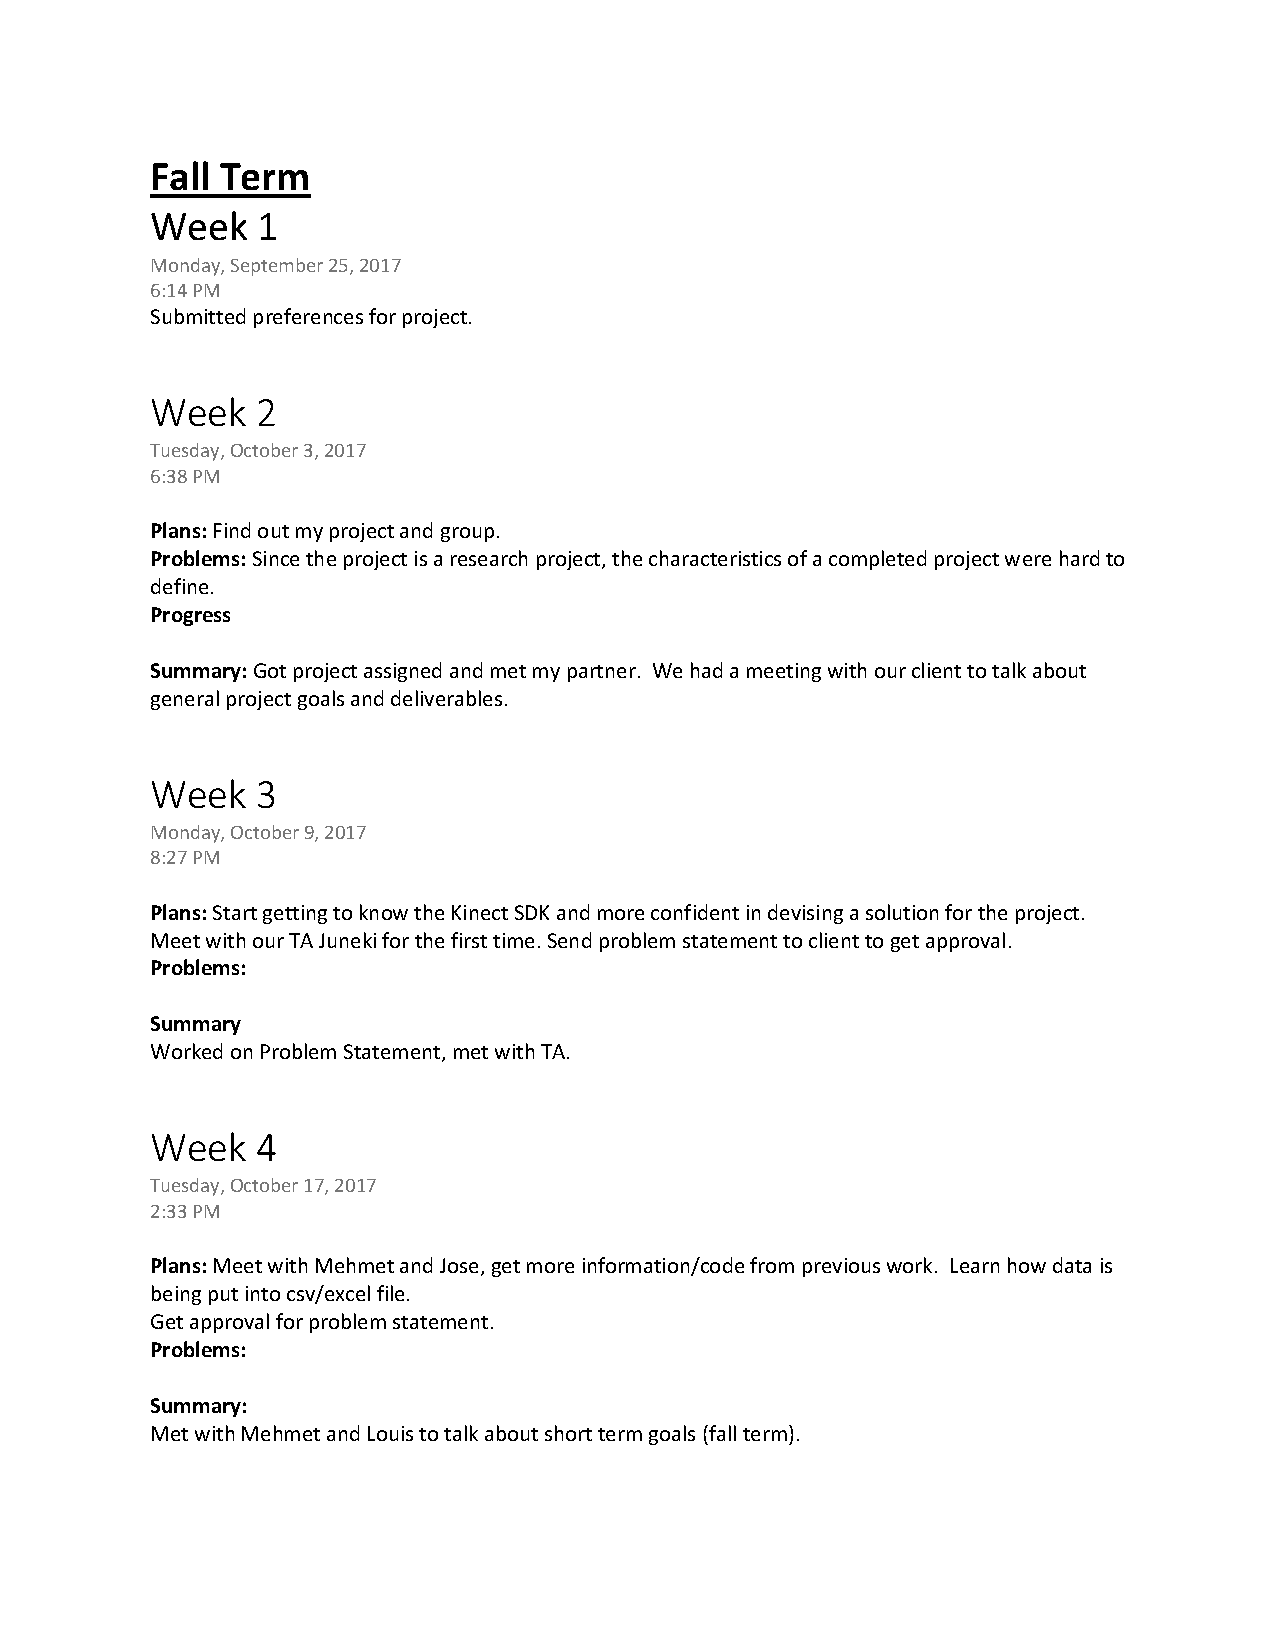
\includepdf[pages=-, pagecommand={}]{requiredDocuments/dimcBlogs}
%%%%%%%%%%%%%%%%%%%%%%%%%%  FINAL EXPO POSTER  %%%%%%%%%%%%%%%%%%%%%%%%
\section{Final Poster}
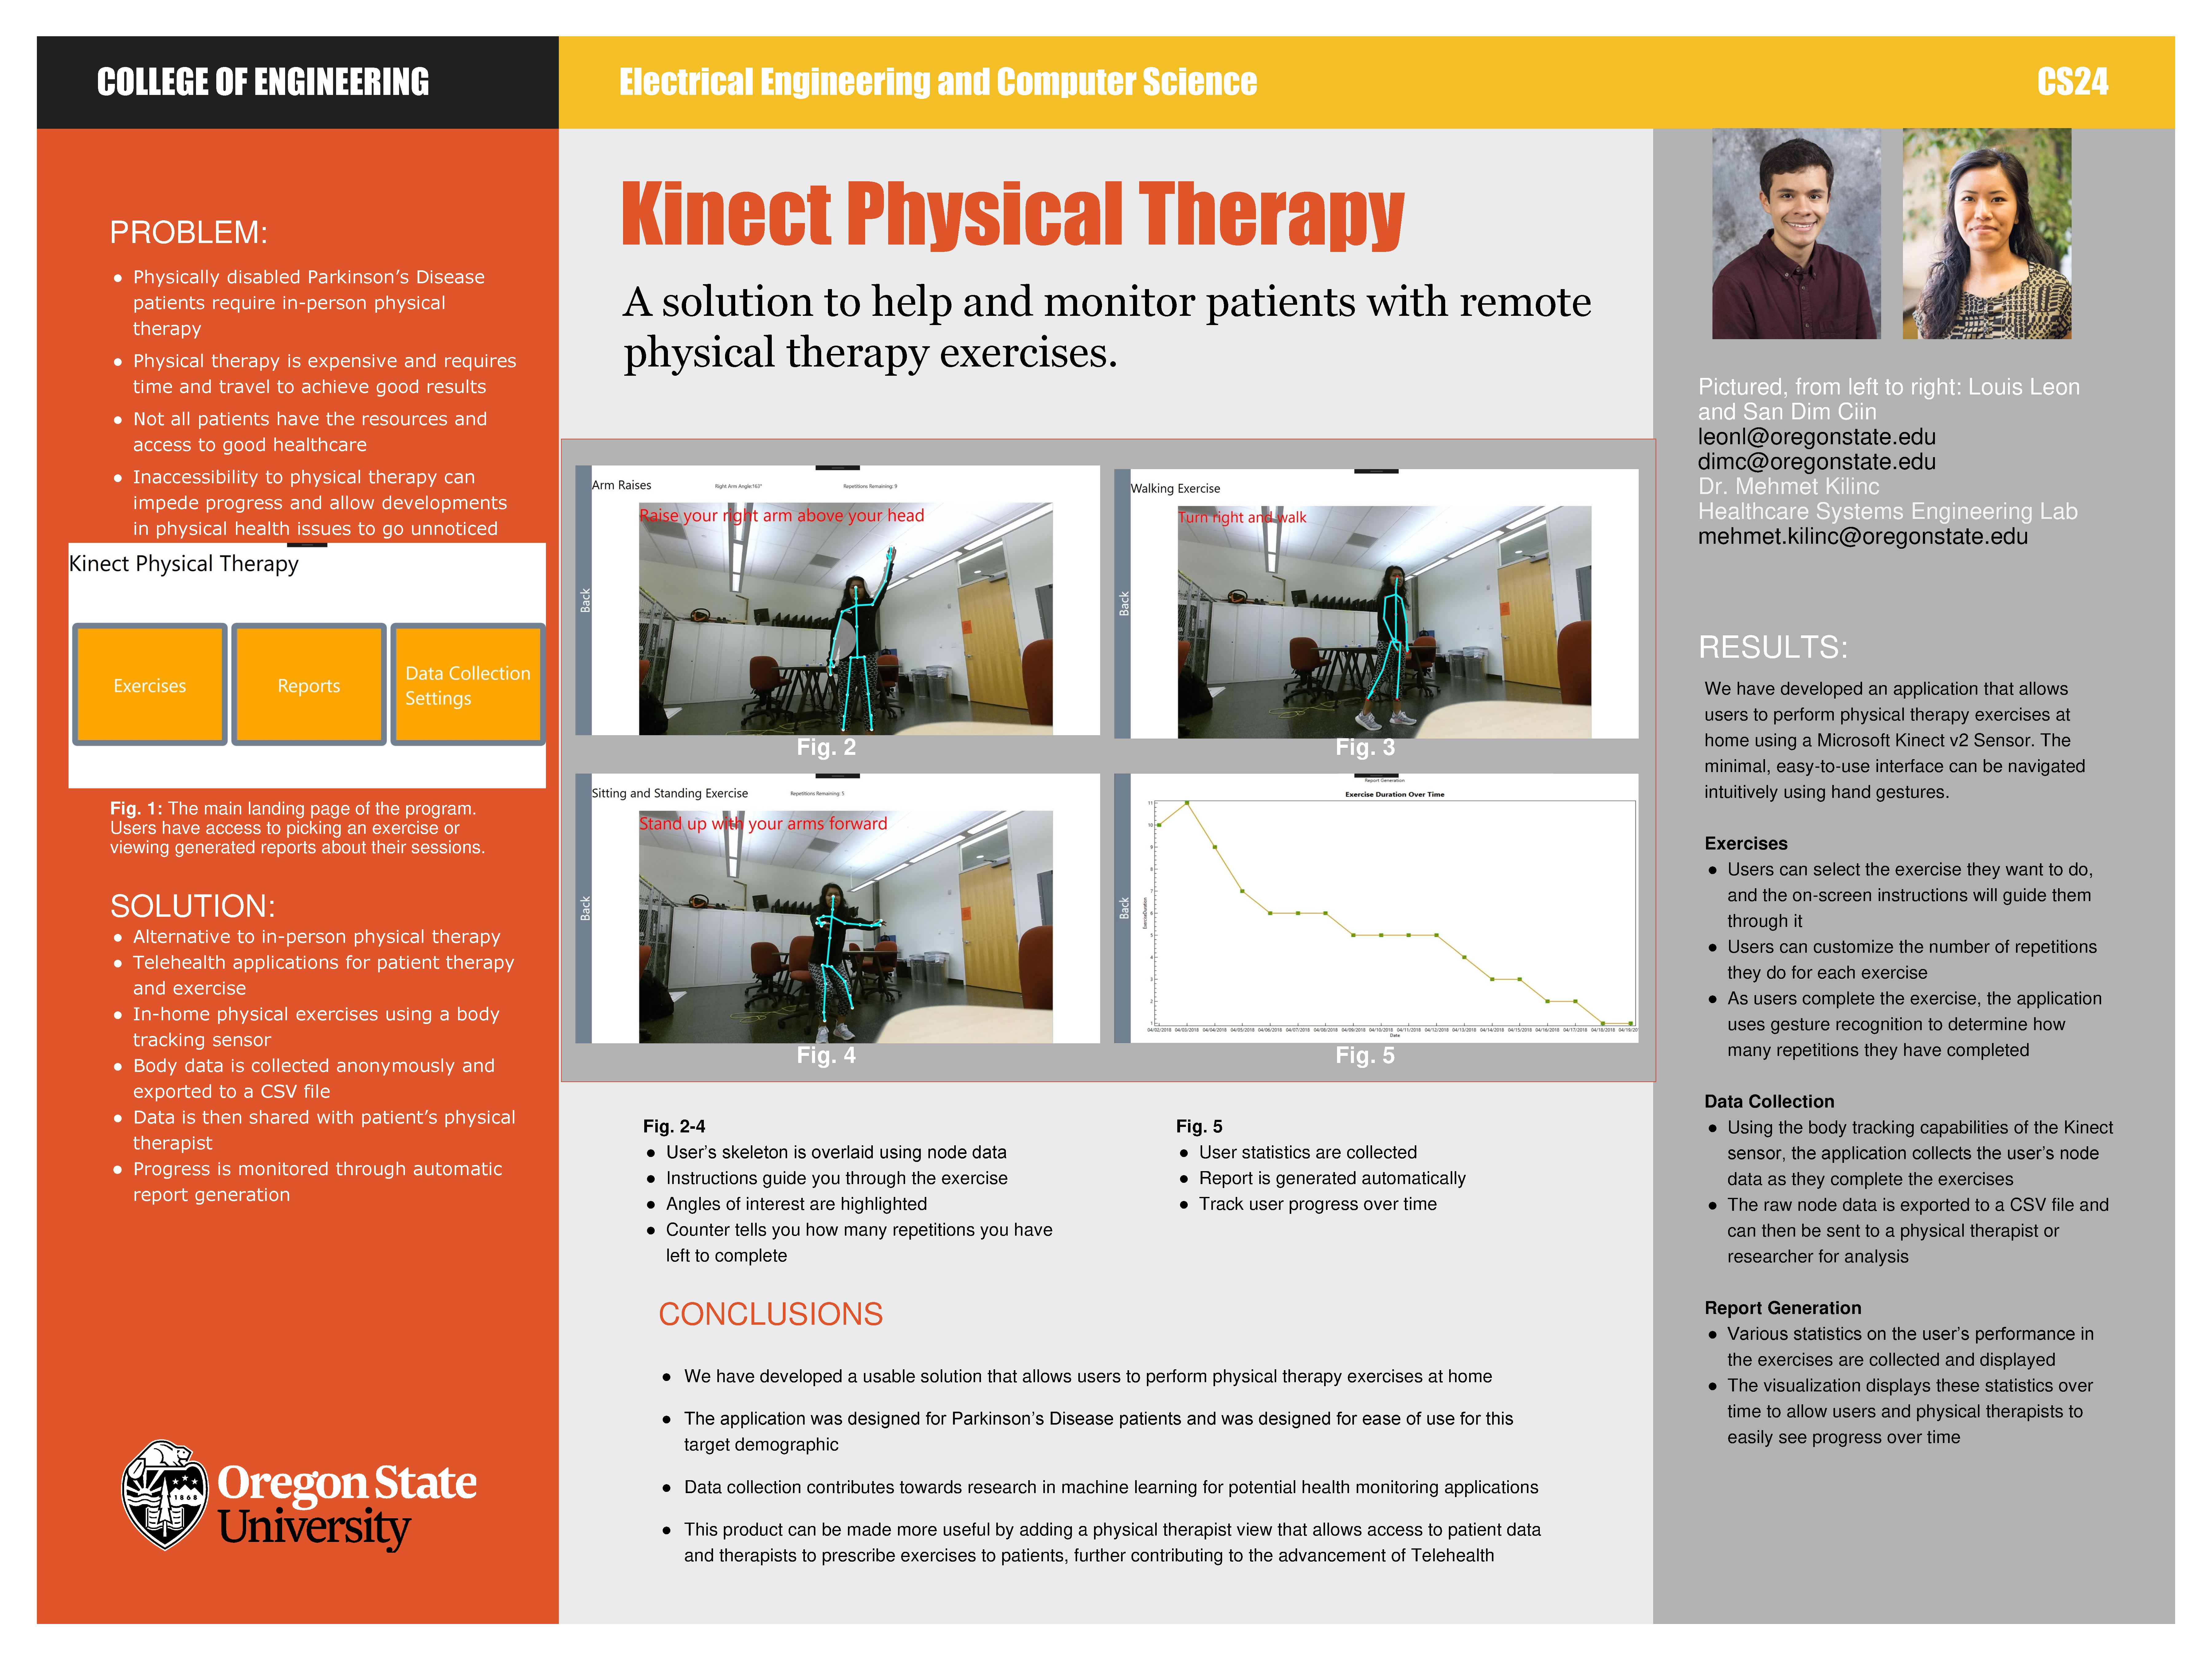
\includepdf[pages=-, pagecommand={},landscape=true]{requiredDocuments/FinalPoster}  
%%%%%%%%%%%%%%%%%%%%%%%%  PROJECT DOCUMENTATION  %%%%%%%%%%%%%%%%%%%%%%
\section{Project Documentation}
\subsection{Structure and Operation}
The directory structure of the project itself includes separate directories for Gestures, Navigation Pages, User Data, Exercise Pages, and Libraries. 

The user interface consists of a main navigation page which allows the user to choose one of three of the following tiles or pages to navigate to: Exercises, Reports, and Settings. Each page has several components and libraries that correspond to it. 

Each exercise option has a dedicated .cs file where the exercise is defined and a corresponding .xaml file for the graphics display. In the exercise files, the Kinect Sensor is initialized along with the exercise gestures, node recorder, and timer. With the use of an open source Kinect library, Vitruvius, the setup for the sensor is greatly simplified. 

The Reports page within the main navigation screen houses the report generation logic. Using a plotting library called OxyPlot, each CSV file containing the user's exercise data for every completed exercise session is processed and plotted onto the display \cite{Vitruvius, KinectDevelop, csvFile}.

\subsection{Installation and Building}

\subsection{System Requirements}
\textbf{Operating System Requirements}
\begin{itemize}
    \item Windows 8 (64-bit) or above
    \item Windows 8.1 (64-bit) or above
    \item Windows Embedded Standard 8 (64-bit)
    \item Windows Embedded Standard 8.1 (64-bit) \cite{KinectConstraints}
\end{itemize}
\textbf{Hardware Requirements}
\begin{itemize}
    \item 64-bit (x64) processor
    \item 4 GB Memory (or more)
    \item Physical dual-core 3.1  GHz (2 logical cores per physical) or faster processor
    \item USB 3.0 controller dedicated to the Kinect for Windows v2 Sensor
    \item A Microsoft Kinect v2 Sensor, which includes a power hub and USB cabling \cite{KinectDevelop,KinectConstraints}
\end{itemize}
\textbf{Runtime Requirements}
\begin{itemize}
    \item .NET Framework 4.0
    \item Kinect v2 SDK
    \item DirectX 11
\end{itemize}
\subsection{User Guide}
\subsubsection{Main Menu Options}
The main menu options displayed when running the application are Exercises, Reports, and Settings. To select one of these options, you must first activate the cursor. Simply raise one open hand in front of you to about shoulder height with your palm facing the sensor and hold it in that position. It should take a couple seconds for a hand icon to appear. Once it appears, move your hand to drag the hand icon cursor over the menu option you would like to select. To select, move your hand forward toward the sensor in a pushing motion. If you would rather use a mouse to navigate, use left click to select.
\subsubsection{Exercises}
To complete an exercise, select the Exercises option. In the Exercise Options menu, select either Arm Raises, Walking, or Sitting and Standing. To begin the exercise, follow the instructions written on the screen. If you are doing the exercise correctly, the repetition counter at the top of the window will count down. Once you have completed the exercise, a dialog box will open. Select a folder and type in a file name for your node data to be saved in. Once the file has been saved, you can navigate away from this page by selecting the Back button.
\subsubsection{Viewing Reports}
To view reports, select the Reports option from the main menu. There are three buttons across the bottom of this page underneath the graphical display. Selecting one of these buttons will display the data for the corresponding exercise.
\subsubsection{Changing Settings}
To customize data collection and exercise repetitions, select the Settings option from the main menu. To specify when to start data collection, select the appropriate radio button on the left side of the page. To specify the duration of data collection, select the units (seconds or minutes) from the drop down box, then type in the integer or decimal value of the duration (30 seconds is the same duration as .5 minutes). To specify the frequency of data collection, type in the frequency (in seconds) of which the node data should be collected. For smaller frequencies of less than one second, the data may not be collected at the specified frequency due to the limitations of the Kinect sensor, but it will not collect node data more frequent than what is specified. To set the repititions for the Arm Raises and Sitting and Standing exercise, enter a whole number into the text box fields. To submit changes, select Submit in the bottom right corner of the page. If a setting is not specified, the default settings will be in place. The default settings are: begin recording when window opens, duration of recording goes until completion of exercise, frequency of recording is the frequency of Kinect sensor node detection, and repititions for both Arm Raises and Sitting and Standing are 10.
%%%%%%%%%%%%%%%%%%%%%%%  RECOMMENDED RESOURCES  %%%%%%%%%%%%%%%%%%%%%%%
\section{Recommended Technical Resources}
\subsection{Useful Websites}
\begin{enumerate}
\item \verb+https://lightbuzz.com/+
\item \verb+https://developer.microsoft.com/en-us/windows/kinect+
\item \verb+https://github.com/LightBuzz/Vitruvius+
\end{enumerate}
%%%%%%%%%%%%%%%%%%%%  CONCLUSIONS AND REFLECTIONS  %%%%%%%%%%%%%%%%%%%%
\section{Conclusions and Reflections}
\begin{flushleft}
{\large\textbf{Louis Leon}\par}
\textbf{What technical information did you learn?}\par
From working on this capstone project, I have learned a lot about programming in the C\# language and using the Kinect SDK to write code that interfaces with the Kinect Sensor architecture. I also learned about using native .NET Framework libraries to access system file paths in order to read and write to files that were essential for the project. I learned more about the Kinect Sensor than I had expected and learned to appreciate the potential of the applications that can be made possible using such a piece of technology. Learning how to develop custom gestures for the Microsoft Kinect was one of my favorite parts of the project \cite{KinectDevelop}. 

\textbf{What non-technical information did you learn?}\par
With the non-technical side of the project, I learned more about neurodegenerative diseases and Parkinson's disease and how they affect the human body as well as why we need certain technologies to help those who suffer from those types of diseases. I learned how physical therapy is used with someone who has Parkinson's disease and what symptoms to look for in a patient. I also gained some experience about what it was like to work on a project with a small team and a client who was expecting and requesting certain requirements of us.

\textbf{What have you learned about project work?}\par
I learned that project work can be extremely rewarding and even more insightful than regular coursework. I learned more about coding in a new language and software development techniques than I have in most courses. I also learned that doing extensive research for a project of this size is essential for doing well and creating a good final product. Also, I experienced what it was like to be able to use existing resources to help develop parts of the project. This allowed us to develop faster without adding any extra complexity to the project and not worrying about debugging that area of the project.

\textbf{What have you learned about project management?}\par
I found that I was able to apply some software engineering skills and other tools learned earlier during my undergraduate courses. The non-technical side of the project was what made development easier and more organized. Researching the topics and libraries used during development was critical because we were able to plan ahead and decide which technology we wanted to implement and how to implement it. I also learned more about the importance of requirement gathering with a client. We wanted to implement as closely to what our client had asked of us and what we thought to be achievable. 

\textbf{What have you learned about working in teams?}\par
When working in teams, I learned how important it was to plan ahead and stay organized and on top of my tasks because some of my work could be required in order to start on other members’ tasks. It was also very beneficial to work together on tasks in person because it motivated me to stay on task and make more progress on the project than it would to work separately. 

\textbf{If you could do it all over, what would you do differently?}\par

\end{flushleft}

\begin{flushleft}
{\large\textbf{San Dim Ciin}\par}
\textbf{What technical information did you learn?}\par
The Microsoft Kinect, along with the .NET framework required to use it, is a technology I was completely new to developing with. To create the user interface, we used Windows Presentation Foundation. This required learning how to write the xaml files to produce the visual aspect of the interface, and I learned how to write C\# code to implement the functionality of the interface. In addition to learning the inner workings of each language, I also learned how to make the visual and functional pieces of the code interact with each other. All of the Kinect functionality was written in the backend portion in C\#. I learned about the many classes in the Kinect SDK that allowed us implement body tracking, gesture recognition, and skeleton display.

\textbf{What non-technical information did you learn?}\par
In addition to the technical information that I learned, I learned about telehealth, physical therapy, and Parkinson's Disease. The product we developed would fit under the category of telehealth, which uses technology to make healthcare more accessible and affordable. Telehealth services can be used to access test results, monitor blood sugar levels, schedule appointments, record physical activity, and much more. When observing a physical therapy session, I learned about various techniques in physical therapy and the meaning behind the way one's body performs actions. For example, when one's stride is short, it means they are struggling with dorsiflexion (the movement of the foot upwards, so that the foot is closer to the shin). I also learned about the causes, symptoms, and treatments of Parkinson's Disease. PD patients exhibit tremors, slow movement, and stiffness, among many other symptoms, due to a disorder of the central nervous system that mainly affects the motor system. 

\textbf{What have you learned about project work?}\par
The main thing I learned about project work is that it is unpredictable. Despite the careful planning and schedule of development, there will always be obstacles that delay our progress. Development requires research of different technologies that we may have not used before, resulting in a learning period and many iterations of trial and error. I also learned the importance of modularization in a project. There were several pieces of our project that went through constant changes. Writing modular code made it possible to keep those changes local and maintain functionality in the project as a whole. Because there were so many frequent changes, I learned that frequent commits to the project repository are necessary for allowing group mates to contribute and make progress on the project. My knowledge of git has increased because of this.

\textbf{What have you learned about project management?}\par
When managing a project, it is important to have long term and short term goals. I learned that long term goals were necessary for evaluating the product and progress made at significant milestones, and short term goals were necessary to keep the team on track and working at a reasonable pace to reach the goals at the milestones. With these goals in mind, I also learned that the schedule of development must be revised when obstacles are encountered that delay progress. When this happens, short term goals change to account for lost time in order to reach the long term goals.

\textbf{What have you learned about working in teams?}\par
In the case of working on a student project, a major aspect of group work is coordinating schedules. Because there was limited overlapping availability, we had to be diligent with planning our meetings ahead of time so that we wouldn't miss opportunities to work together. We would meet at most three times a week, so we had a set of tasks to complete for each session to keep us on track. The benefit of working in groups is being able to allocate tasks to each member. We had to have a level of trust in each other to complete tasks that we worked on individually. This allowed us to be focused on our task and ask the other for help when we needed it. With this dynamic, we were able to make consistent progress and put our energy into doing our part instead of babysitting the other group mate.

\textbf{If you could do it all over, what would you do differently?}\par
If I could do it all over, I would begin development much sooner. This would have allowed a buffer for setbacks and time for learning of new technologies. I also would have made the plan for the final product much more concrete at the very beginning. While we were able to accomplish everything laid out in our documents, I was still unsure about what would please our client throughout the process. The requirements given to us by our client weren't very strict or specific, so we had a bit of freedom with what we wanted to implement. Because of this, I never had a solid idea of what a final product should be.

\end{flushleft}
%%%%%%%%%%%%%%%%%%%%%%%%%%  APPENDIX I  %%%%%%%%%%%%%%%%%%%%%%%%%%%%%%%

\section{Appendix I: Essential Code Listings}
\begin{figure}[H]
\begin{lstlisting}[language=C, style=customc]
 public PlotModel OpenTimes(string file)
        {
            var doc = new CsvDocument();
            doc.Load(file);
            var tmp = new PlotModel { Title = "Exercise Duration Over Time" };
            tmp.IsLegendVisible = false;
            tmp.PlotMargins = new OxyThickness(50, 0, 0, 40);
            for (int i = 1; i < doc.Headers.Length; i++)
            {
                var ls = new ScatterSeries { Title = doc.Headers[i] };
                foreach (var item in doc.Items)
                {
                    var t1 = DateTime.Parse(item[0]);
                    var t2 = DateTime.Parse(item[i]);
                    double x = DateTimeAxis.ToDouble(t2);
                    double y = DateTimeAxis.ToDouble(t1.Minute);
                    ls.Points.Add(new ScatterPoint(x, y));
                }
                tmp.Series.Add(ls);
            }
            for (int i = 1; i < doc.Headers.Length; i++)
            {
                var ls = new LineSeries { Title = doc.Headers[i] };
                foreach (var item in doc.Items)
                {
                    var t1 = DateTime.Parse(item[0]);
                    var t2 = DateTime.Parse(item[i]);
                    double x = DateTimeAxis.ToDouble(t2);
                    double y = DateTimeAxis.ToDouble(t1.Minute);
                    ls.Points.Add(new DataPoint(x, y));
                }
                tmp.Series.Add(ls);
            }
            tmp.Axes.Add(new LinearAxis
            {
                Position = AxisPosition.Left,
                Title = doc.Headers[0],
                TickStyle = TickStyle.Inside,
            });
            tmp.Axes.Add(new DateTimeAxis
            {
                Position = AxisPosition.Bottom,
                Title = doc.Headers[1],
                TickStyle = TickStyle.Inside,
                StringFormat = "MM/dd/yyyy"
            });
            return tmp;
        }
\end{lstlisting}
\caption{Report Generation with OxyPlot}
\end{figure}
%%%%%%%%%%%%%%%%%%%%%%%%%%%%%%  APPENDIX II  %%%%%%%%%%%%%%%%%%%%%%%%%%
\section{Appendix II: Related Project Information}

%%%%%%%%%%%%%%%%%%%%%%%%%%%%%  BIBLIOGRAPHY  %%%%%%%%%%%%%%%%%%%%%%%%%%
\bibliographystyle{ieeetr}
\bibliography{FinalReport}
\end{document}
